% Discretizations in ug4

\begin {frame} [t]
\frametitle {``Global'' assembling}
\centerline {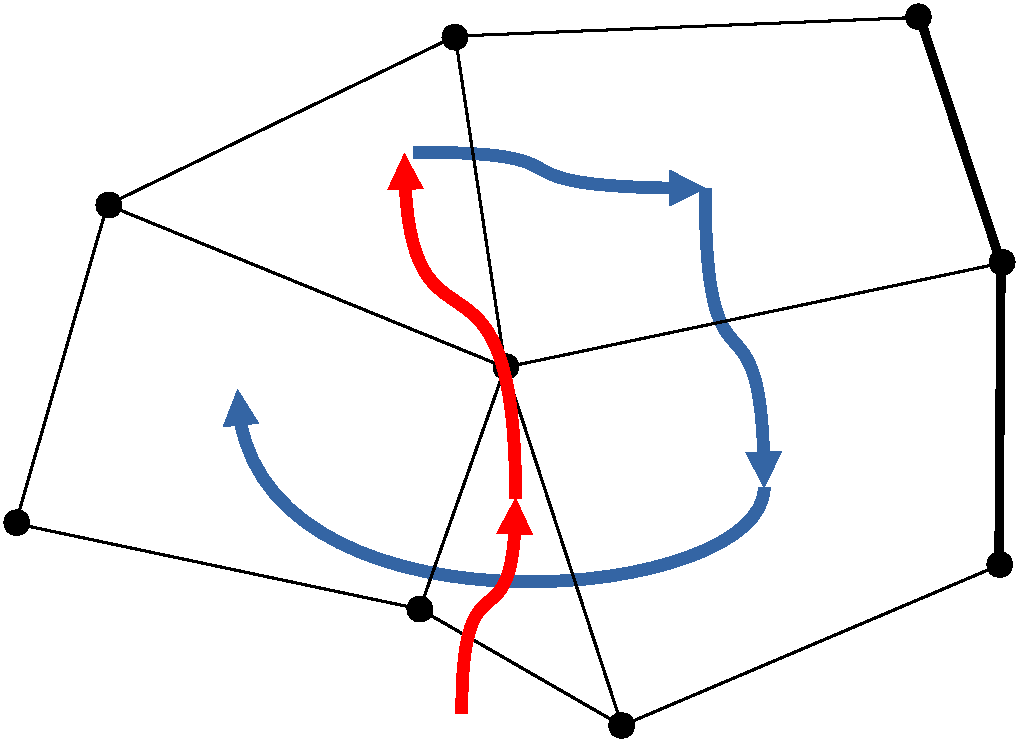
\includegraphics [width=0.6\textwidth] {DiscDetails-Global.pdf}}
The cycle over all the grids elements and summing up the contributions is referred to as
``global assembling'' (``{\color{blue} DomainDiscretization}'' class in ug4).
DomainDiscretization calls ``local discretizations'' for every element. This
loop is subdivided into the loops over {\color{blue} element types}, subdomains
(``{\color{blue} subsets}''), \dots
\end {frame}

\begin {frame} [t]
\frametitle {``Local'' assembling}
\centerline {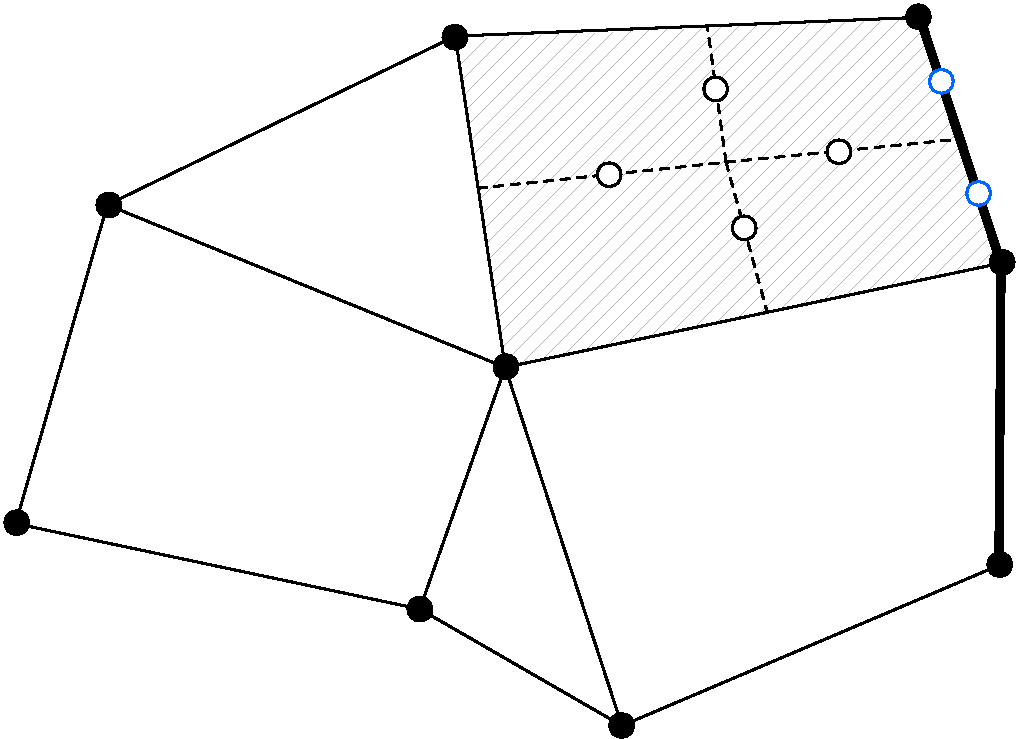
\includegraphics [width=0.6\textwidth] {DiscDetails-Local.pdf}}
In every full-dimensional grid element, one uses the shape functions and the
geometrical information to evaluate the local contributions. These computations
are called ``local assembling'' (``derived from {\color{blue} ElemDisc}'' in ug4).
This requires the problem coefficients (like $d(x)$).
\end {frame}

\begin {frame} [t]
\frametitle {Equations and boundary conditions}
\centerline {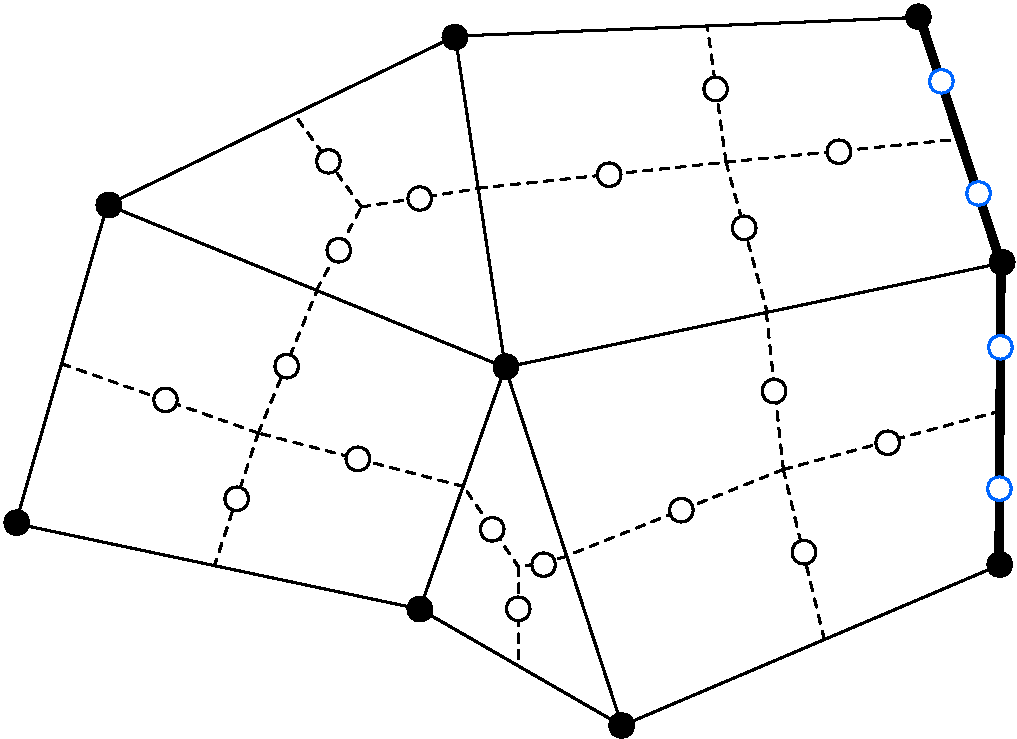
\includegraphics [width=0.6\textwidth] {DiscDetails-Entire.pdf}}
After the global loop, the complete matrix and defect are assembled. Boundary conditions
should be implemented either as ElemDisc's (e.g.\ the Neumann BC) or as \emph{constraints}
(e.g.\ Dirichlet BC). DomainDiscretization (and standard BC) are implemented in ugcore.
Local discretizations are normally implemented in plugins (e.g.\ ConvectionDiffusion).
\end {frame}

\begin {frame} [t]
\frametitle {Solver objects: A non-linear model}
\centerline {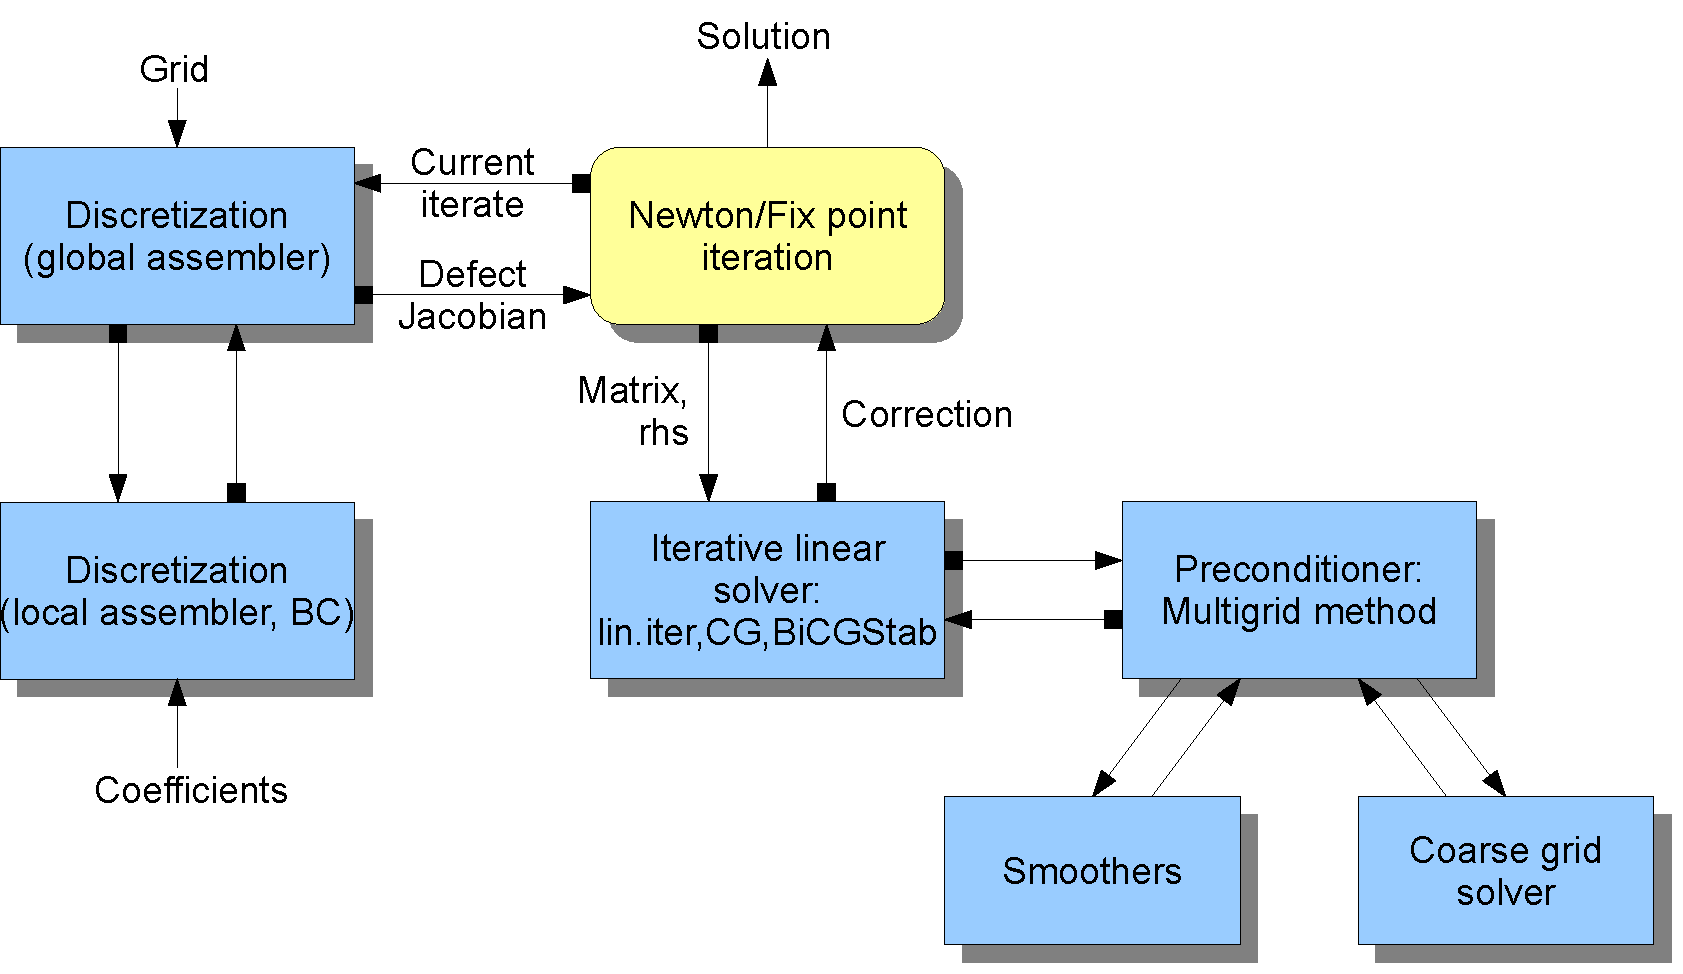
\includegraphics [width=1.15\textwidth] {StationarySolverFull}}
\end {frame}

% End of File
